\chapter{Standar Kompetensi Lulusan}

\section{Profil Lulusan}

Profil lulusan Program Studi D4 Teknik Informatika ditetapkan melalui diskusi dengan program studi sejenis di perguruan tinggi lain, yaitu Politeknik Negeri Jember (POLIJE), Politeknik Elektronika Negeri Surabaya (PENS), dan Politeknik Negeri Semarang (POLINES). Dari profil lulusan yang disepakati, selanjutnya diturunkan Capaian Pembelajaran Lulusan (CPL) yang mengacu pada Standar Nasional Pendidikan Tinggi (SN-Dikti) untuk unsur sikap dan keterampilan umum, serta Kerangka Kualifikasi Nasional Indonesia (KKNI) level 6 untuk unsur keterampilan khusus dan pengetahuan.

\textit{Profil lulusan berikut diadopsi dari Dokumen Kurikulum D4 Teknik Informatika 2020 (4 profil: IT Project Manager, IT Team Leader, Programmer, System Analyst). Profil lulusan beserta pemetaannya ke kode CPL 2025 pada setiap profil telah ditetapkan dan divalidasi oleh tim kurikulum.}

\subsection{IT Project Manager}

Lulusan dengan profil IT Project Manager memiliki kompetensi:
\begin{itemize}
\item Mampu menyesuaikan penyelesaian proyek dengan \textit{framework}/alat tradisional (\textit{waterfall}) atau \textit{Agile}.
\item Mampu mengestimasi waktu (\textit{timing}) dalam rencana proyek yang dibuat.
\item Memiliki kemampuan mengarahkan dan memotivasi anggota tim proyek, serta kemampuan negosiasi, pemecahan masalah, komunikasi, dan interpersonal.
\item Mampu mengimplementasikan strategi dan ilmu industri, serta memiliki kemampuan komunikasi yang baik dengan seluruh pihak yang terlibat dalam proyek seperti klien, vendor, dan anggota tim.
\item Mampu memprediksi masalah yang mungkin muncul beserta solusinya, serta memiliki rencana alternatif atau cadangan ketika menemui permasalahan (\textit{problem solving}).
\item Memiliki pengetahuan mengenai analisis biaya proyek.
\item Memiliki kemampuan mengidentifikasi, merencanakan, dan mengelola risiko proyek.
\item Memahami metode \textit{project management}.
\end{itemize}
Pemetaan CPL yang relevan: CPL03, CPL08.

\subsection{IT Team Leader}

Lulusan dengan profil IT Team Leader memiliki kompetensi:
\begin{itemize}
\item Memiliki kemampuan mengoordinasikan dan mendelegasikan tanggung jawab tim TI.
\item Mampu menginspirasi tim melalui diskusi yang terbuka, jujur, dan transparan, berfokus pada strategi dan visi teknologi.
\item Memiliki pengetahuan serta pengalaman dalam proyek yang dijalankan, terkait metode, \textit{tools}, dan \textit{software}.
\item Memiliki kemampuan menentukan waktu pengerjaan proyek, pelaporan hasil, dan cara penyelesaian permasalahan.
\item Memiliki kemampuan berkomunikasi yang baik dengan seluruh pihak yang terlibat dalam proyek.
\item Mampu menerjemahkan \textit{business process} sebuah proyek untuk diimplementasikan ke dalam aplikasi (\textit{software}).
\item Memiliki kemampuan teknis yang meliputi \textit{tools}, bahasa pemrograman, dan basis data yang digunakan dalam mengembangkan proyek.
\item Mampu memberikan solusi terhadap permasalahan teknis maupun nonteknis yang dihadapi anggota tim, serta memiliki kemampuan berpikir kritis.
\item Memiliki kemampuan menjembatani kebutuhan antara tim produk dan tim developer.
\item Mampu menganalisis spesifikasi dan permintaan dari tim produk.
\item Mampu menjelaskan secara teknis tugas yang perlu dilakukan oleh tim \textit{Backend Engineer}, \textit{Frontend Engineer}, dan \textit{Quality Assurance} agar sesuai dengan ekspektasi tim produk.
\item Memiliki kemampuan dan pemahaman dari sisi \textit{coding} serta kemampuan dalam bidang arsitektur sistem.
\item Memiliki pemahaman terhadap struktur basis data.
\item Memiliki wawasan terhadap \textit{tech stack} yang dapat diterapkan agar proyek sesuai dengan persyaratan yang diinginkan.
\end{itemize}
Pemetaan CPL yang relevan: CPL02, CPL03, CPL06.

\subsection{Programmer (Web, Desktop, Mobile, Multimedia)}

Lulusan dengan profil Programmer memiliki kompetensi:
\begin{itemize}
\item Memiliki kemampuan menulis program perangkat lunak.
\item Memiliki kemampuan mentransformasikan rancangan program yang dibuat oleh \textit{software designer}/\textit{engineer}/\textit{system analyst} menjadi instruksi-instruksi yang dapat dikerjakan oleh komputer.
\item Dapat membaca \textit{source code} sebuah aplikasi yang akan/sedang dikembangkan, serta memiliki kemampuan mencari \textit{bug} atau kesalahan dari program yang telah dibuat sebelumnya.
\item Memiliki kemampuan membaca dokumentasi untuk mengenal setiap kode dari masing-masing bahasa pemrograman yang digunakan.
\item Memiliki kemampuan mempelajari beberapa bahasa pemrograman.
\item Memiliki kemampuan multitasking dalam mengintegrasikan berbagai lapisan teknologi.
\item Memiliki kemampuan berbahasa Inggris dengan baik untuk memahami pesan \textit{error}, membaca dokumentasi, bertanya di forum global, dan mencari referensi berbahasa Inggris.
\item Mampu mempelajari konsep dan menerapkannya pada permasalahan lain.
\item Memiliki pemahaman tentang aljabar dan aritmetika.
\item Memiliki kemampuan mengidentifikasi masalah dan menemukan cara paling efisien untuk menyelesaikannya melalui pemrograman.
\item Memiliki kemampuan komunikasi yang baik.
\item Mampu bekerja sama dalam tim, serta memiliki kemampuan merancang struktur program sejak penulisan baris kode pertama.
\item Memiliki kemauan untuk terus belajar mengenai hal-hal baru.
\end{itemize}
Pemetaan CPL yang relevan: CPL02, CPL09, CPL10.

\subsection{System Analyst}

Lulusan dengan profil System Analyst memiliki kompetensi:
\begin{itemize}
\item Memiliki pengetahuan tentang sistem operasi yang umum, bahasa pemrograman, dan platform perangkat keras.
\item Memiliki pengetahuan mengenai \textit{business process mapping}, \textit{software development}, dan \textit{project management}.
\item Memiliki kemampuan mengidentifikasi masalah, mempertimbangkan solusi, mengimplementasikan rencana, dan mengevaluasi perbaikan yang ada.
\item Mampu mengomunikasikan informasi teknis agar dapat dipahami klien, serta memiliki kemampuan menganalisis pilihan produk dan menemukan inovasi sistem yang paling ekonomis maupun aman bagi perusahaan.
\item Mampu membuat kerangka rencana mengenai bagaimana produk akan terlihat serta memastikan seluruh detail rencana dan tahapan dieksekusi dengan baik.
\item Menguasai metodologi pengembangan sistem serta mampu memprediksi faktor eksternal seperti kenaikan harga perangkat atau munculnya pesaing.
\item Menguasai perangkat lunak maupun perangkat keras terbaru beserta keunggulan dan batasannya, serta memiliki keahlian komunikasi/interpersonal.
\item Memiliki pengetahuan dan keterampilan teknologi komputer, bahasa pemrograman, dan teknik pengolahan data.
\item Memiliki pengetahuan tentang metode kuantitatif seperti \textit{linear programming}, \textit{dynamic programming}, regresi, jaringan, \textit{decision tree}, tren, dan simulasi.
\item Memiliki kemampuan menganalisis masalah dan memberikan solusi, serta kemampuan komunikasi verbal maupun tulisan untuk membina dan menjaga hubungan.
\end{itemize}
Pemetaan CPL yang relevan: CPL04, CPL05, CPL10.

\section{Capaian Pembelajaran Lulusan}

\begin{longtable}{L{2.2cm}L{11.8cm}}
\toprule
Kode & Deskripsi CPL \\
\midrule
\endhead
CPL01 & Menginternalisasi ketakwaan kepada Tuhan Yang Maha Esa, menaati hukum, disiplin, dan menunjukkan profesionalisme melalui etika profesi, pembelajaran sepanjang hayat, serta respons terhadap isu sosial dan teknologi. \\
CPL02 & Menguasai konsep teoritis bidang pengetahuan mengenai berbagai prinsip rekayasa sistem/perangkat lunak dalam merancang solusi aplikasi multi-platform yang relevan dengan kebutuhan stakeholder. \\
CPL03 & Mampu mengelola tim, manajemen diri, berkomunikasi secara lisan maupun tertulis dengan baik dan mampu melakukan presentasi. \\
CPL04 & Mampu menyusun deskripsi saintifik hasil kajian implikasi pengembangan atau implementasi ilmu pengetahuan teknologi dalam bentuk skripsi atau laporan tugas akhir atau artikel ilmiah. \\
CPL05 & Mampu menerapkan solusi teknologi komputasi dan infrastruktur digital dengan mempertimbangkan berbagai teknik/pendekatan yang sesuai dengan kebutuhan. \\
CPL06 & Mampu merancang, mengimplementasikan, menguji, melakukan deployment, dan memelihara, serta menjamin mutu perangkat lunak yang menjawab permasalahan dan memenuhi kebutuhan stakeholder. \\
CPL07 & Mampu mengembangkan sistem komputasi cerdas, analisis data dengan menerapkan algoritma dan teknik kecerdasan artifisial secara tepat guna. \\
CPL08 & Mampu mengelola proyek teknologi informasi secara profesional dengan mengoptimalkan sumber daya yang tersedia. \\
CPL09 & Memiliki pemahaman yang memadai terkait cara kerja sistem komputer dan berbagai teknik/pendekatan berbasis komputasi untuk memecahkan masalah stakeholder. \\
CPL10 & Memiliki kompetensi untuk menganalisis persoalan kompleks untuk mengidentifikasi solusi bidang informatika/ilmu komputer dengan mempertimbangkan wawasan ilmu multidisiplin. \\
\bottomrule
\end{longtable}

\section{CPMK per CPL}

\subsection{CPL01}
\begin{longtable}{L{2cm}L{12cm}}
\toprule
CPMK & Deskripsi \\
\midrule
\endhead
CPMK0101 & Mampu menunjukkan profesionalisme melalui penerapan etika profesi TI, keselamatan kerja, kewirausahaan bertanggung jawab, rekayasa perangkat lunak ramah lingkungan, dan disiplin dalam penelitian maupun penerapan aplikasi teknologi. \\
CPMK0102 & Mampu menginternalisasi nilai ketakwaan kepada Tuhan YME, Pancasila, kewarganegaraan, dan menunjukkan pembelajaran sepanjang hayat melalui disiplin diri, tanggung jawab sosial, dan adaptasi karir profesional. \\
\bottomrule
\end{longtable}

\subsection{CPL02}
\begin{longtable}{L{2cm}L{12cm}}
\toprule
CPMK & Deskripsi \\
\midrule
\endhead
CPMK0201 & Mampu merancang dan mendokumentasikan rencana manajemen proyek pengembangan aplikasi multi-platform dengan menerapkan metodologi pengembangan perangkat lunak yang tepat. \\
CPMK0202 & Mampu menerapkan prinsip dan metode User Experience (UX) Design untuk merancang prototipe antarmuka aplikasi multi-platform yang interaktif. \\
CPMK0203 & Mampu merancang skema dan arsitektur manajemen data yang efektif dan terstruktur untuk mendukung solusi aplikasi multi-platform. \\
CPMK0204 & Mampu menganalisis kebutuhan komputasi dari sebuah solusi IoT multi-platform dan arsitektur terdistribusi. \\
CPMK0205 & Mampu menerapkan prinsip dan pola desain perangkat lunak untuk membuat blueprint arsitektural dan komponen solusi aplikasi multi-platform yang modular, maintainable, dan scalable. \\
CPMK0206 & Mampu menganalisis karakteristik dan kebutuhan sumber daya dari aplikasi multi-platform, lalu merancang strategi manajemen sumber daya sistem. \\
CPMK0207 & Mampu menganalisis kompleksitas permasalahan komputasi kemudian memilih dan merancang struktur data serta algoritma yang optimal. \\
CPMK0208 & Mampu menganalisis kebutuhan komputasi dari solusi aplikasi multi-platform dan memilih arsitektur computing system yang sesuai. \\
CPMK0209 & Mampu memilih dan menerapkan arsitektur serta teknologi pengembangan berbasis platform yang tepat untuk solusi aplikasi multi-platform. \\
CPMK0210 & Mampu menerapkan prinsip fundamental rekayasa perangkat lunak dan paradigma berorientasi objek dalam merancang spesifikasi teknis. \\
CPMK0211 & Mampu menerapkan metodologi analisis dan desain sistem secara terstruktur untuk mentransformasi kebutuhan stakeholder menjadi spesifikasi teknis yang komprehensif. \\
\bottomrule
\end{longtable}

\subsection{CPL03}
\begin{longtable}{L{2cm}L{12cm}}
\toprule
CPMK & Deskripsi \\
\midrule
\endhead
CPMK0301 & Mampu mengelola diri secara profesional, berkomunikasi secara lisan maupun tertulis, dan melakukan presentasi secara efektif dalam konteks kerja. \\
CPMK0302 & Mampu mengelola tim dan proyek secara terencana, mulai dari perencanaan, koordinasi, komunikasi antar anggota, hingga penyampaian hasil kepada pemangku kepentingan. \\
CPMK0303 & Mampu mengembangkan diri secara berkelanjutan melalui komunikasi profesional, presentasi diri, dan pengelolaan karir jangka panjang. \\
\bottomrule
\end{longtable}

\subsection{CPL04}
\begin{longtable}{L{2cm}L{12cm}}
\toprule
CPMK & Deskripsi \\
\midrule
\endhead
CPMK0401 & Mampu menganalisis masalah kompleks dan menyusun solusi rasional berbasis data dalam bentuk deskripsi ilmiah yang terstruktur. \\
CPMK0402 & Mampu mendokumentasikan proyek teknologi informasi secara sistematis dalam laporan teknis yang sesuai standar. \\
CPMK0403 & Mampu merumuskan masalah penelitian, menyusun metode, membuat proposal, dan menuliskan deskripsi ilmiah yang koheren. \\
CPMK0404 & Mampu melaksanakan penelitian dan menuliskan hasilnya dalam bentuk skripsi, laporan tugas akhir, atau artikel ilmiah. \\
\bottomrule
\end{longtable}

\subsection{CPL05}
\begin{longtable}{L{2cm}L{12cm}}
\toprule
CPMK & Deskripsi \\
\midrule
\endhead
CPMK0501 & Mampu merumuskan kebijakan dan prosedur keamanan infrastruktur jaringan dan layanan cloud. \\
CPMK0502 & Mampu mengidentifikasi dan menangani isu keamanan pada sistem operasi, jaringan komputer, dan platform cloud. \\
CPMK0503 & Mampu merancang dan menerapkan solusi komputasi paralel dan terdistribusi untuk kebutuhan IoT, Big Data, dan cloud. \\
CPMK0504 & Mampu merancang arsitektur, protokol, dan konfigurasi infrastruktur jaringan komputer sesuai kebutuhan. \\
CPMK0505 & Mampu menerapkan mekanisme keamanan jaringan untuk melindungi data dan layanan dari ancaman. \\
CPMK0508 & Mampu menerapkan prinsip \textit{information assurance} dan \textit{software security} dalam pengembangan sistem. \\
CPMK0509 & Mampu merancang dan mengelola layanan komputasi virtual yang efisien, \textit{scalable}, dan berkelanjutan. \\
\bottomrule
\end{longtable}

\subsection{CPL06}
\begin{longtable}{L{2cm}L{12cm}}
\toprule
CPMK & Deskripsi \\
\midrule
\endhead
CPMK0601 & Mampu menerapkan prinsip UX dan quality assurance untuk meningkatkan pengalaman pengguna pada perangkat lunak. \\
CPMK0602 & Mampu merancang komponen perangkat lunak menggunakan \textit{software design pattern} yang modular dan terpelihara. \\
CPMK0603 & Mampu mengimplementasikan dan melakukan \textit{deployment} aplikasi berbasis web, mobile, maupun framework pilihan. \\
CPMK0605 & Mampu mengembangkan dan memelihara kualitas kode perangkat lunak sesuai standar yang berlaku. \\
CPMK0606 & Mampu menyusun proses \textit{deployment} dan rencana pemeliharaan perangkat lunak berbasis siklus hidup pengembangan (SDLC). \\
CPMK0607 & Mampu membangun solusi sistem informasi terintegrasi yang kompleks dan menjawab kebutuhan \textit{stakeholder}. \\
CPMK0608 & Mampu menyusun strategi pengujian, verifikasi, validasi, dan jaminan mutu perangkat lunak secara sistematis. \\
CPMK0609 & Mampu melakukan \textit{software modeling and analysis} yang akurat sebagai dasar pengembangan perangkat lunak berkualitas. \\
\bottomrule
\end{longtable}

\subsection{CPL07}
\begin{longtable}{L{2cm}L{12cm}}
\toprule
CPMK & Deskripsi \\
\midrule
\endhead
CPMK0701 & Mampu membangun sistem manajemen data yang handal untuk penyimpanan dan pengelolaan informasi skala besar. \\
CPMK0702 & Mampu melakukan pemrosesan data skala besar menggunakan arsitektur komputasi paralel dan terdistribusi. \\
CPMK0703 & Mampu merancang struktur data dan algoritma yang efisien untuk kebutuhan pengolahan data. \\
CPMK0704 & Mampu memanfaatkan berbagai bahasa dan paradigma pemrograman yang sesuai untuk menyelesaikan masalah komputasi. \\
CPMK0705 & Mampu melakukan pengolahan citra dan visualisasi data menggunakan teknik yang tepat guna. \\
CPMK0706 & Mampu mengembangkan sistem cerdas berbasis AI dan \textit{machine learning} untuk analisis data dan pengambilan keputusan. \\
CPMK0707 & Mampu melakukan pemodelan dan simulasi menggunakan pendekatan statistika komputasi atau metode numerik. \\
CPMK0708 & Mampu memilih dan menerapkan struktur data yang tepat untuk menghasilkan solusi komputasi yang efisien. \\
\bottomrule
\end{longtable}

\subsection{CPL08}
\begin{longtable}{L{2cm}L{12cm}}
\toprule
CPMK & Deskripsi \\
\midrule
\endhead
CPMK0801 & Mampu menyusun rencana proyek teknologi informasi mencakup estimasi biaya, jadwal, alokasi sumber daya, dan manajemen risiko. \\
CPMK0802 & Mampu menerapkan rekayasa perangkat lunak dan UI/UX dalam siklus hidup proyek disertai penjaminan kualitas perangkat lunak (SQA). \\
CPMK0803 & Mampu melaksanakan, memonitor, dan mengendalikan proyek serta mengelola dinamika tim secara efektif. \\
CPMK0804 & Mampu mendemonstrasikan pengelolaan proyek secara utuh dalam konteks riset maupun industri hingga tahap penyelesaian. \\
\bottomrule
\end{longtable}

\subsection{CPL09}
\begin{longtable}{L{2cm}L{12cm}}
\toprule
CPMK & Deskripsi \\
\midrule
\endhead
CPMK0901 & Mampu menjelaskan cara kerja sistem komputer dan komponen utamanya secara komprehensif. \\
CPMK0902 & Mampu menerapkan prinsip matematis dan struktur diskrit untuk keperluan analisis komputasional. \\
CPMK0903 & Mampu menerapkan logika komputasi, pemrograman dasar, dan perancangan algoritma untuk memecahkan masalah. \\
CPMK0904 & Mampu menjelaskan prinsip kerja sistem komputasi paralel dan terdistribusi pada pemrosesan data skala besar. \\
CPMK0905 & Mampu menerapkan konsep virtualisasi dan \textit{cloud computing} dalam lingkungan komputasi modern. \\
\bottomrule
\end{longtable}

\subsection{CPL10}
\begin{longtable}{L{2cm}L{12cm}}
\toprule
CPMK & Deskripsi \\
\midrule
\endhead
CPMK1001 & Mampu merancang solusi basis data yang tepat untuk menyelesaikan persoalan kompleks pengelolaan data dan informasi. \\
CPMK1002 & Mampu merancang mekanisme keamanan jaringan untuk melindungi data dan layanan dari ancaman multidisiplin. \\
CPMK1003 & Mampu membangun solusi jaringan \textit{on-premise} maupun berbasis \textit{cloud} yang andal, aman, dan \textit{scalable}. \\
CPMK1004 & Mampu melakukan visualisasi dan representasi grafis data sebagai dasar analisis dan pengambilan keputusan. \\
CPMK1005 & Mampu mengevaluasi solusi sistem cerdas berdasarkan kinerja, keandalan, dan interpretabilitas model. \\
CPMK1006 & Mampu mengevaluasi dan mengembangkan aplikasi web dan mobile sesuai kebutuhan pengguna dan industri. \\
CPMK1007 & Mampu menghasilkan solusi numerik berbasis struktur diskrit untuk persoalan komputasi tertentu. \\
CPMK1008 & Mampu mengintegrasikan hasil analisis dan desain sistem ke dalam proses pengembangan perangkat lunak secara koheren. \\
CPMK1009 & Mampu mengidentifikasi tahapan penyelesaian ilmiah yang tepat untuk persoalan kompleks di bidang informatika. \\
\bottomrule
\end{longtable}

\section{Analisis Ketercapaian CPL}

\subsection{Ringkasan Eksekutif}

Bagian ini menyajikan analisis ketercapaian Capaian Pembelajaran Lulusan (CPL) berdasarkan data nilai riil mahasiswa, disusun untuk Ketua Program Studi (KPS) pada 13 Juli 2026. Sumber data adalah basis data nilai \texttt{nilai\_staging}, dipetakan ke taksonomi kurikulum resmi pada \texttt{obe\_system} (Kurikulum 2025). Sebanyak 18.982 nilai mata kuliah (tahun akademik 2021/2022 dan 2022/2023) berhasil dipetakan 100\% ke taksonomi resmi (10 CPL, 56 MK, 83 CPMK). Ketercapaian CPL dihitung sebagai rata-rata tertimbang untuk 5 angkatan aktif (2018--2022): nilai satu mata kuliah dibagi rata ke seluruh CPMK mata kuliah tersebut, kemudian diagregasi ke CPL. Rata-rata capaian berkisar antara 67\% hingga 82\%, dengan tingkat pencapaian ambang minimal (\(\geq 50{,}01\)) sebesar 92\% hingga 99,9\%.

\textit{Analisis ini bersifat \textbf{read-only}; angka pada bagian ini belum diendapkan ke basis data produksi \texttt{obe\_system}. Terdapat empat keterbatasan metodologis yang wajib disertakan pada dokumen akreditasi (lihat Subbagian~\ref{subsec:cpl-keterbatasan}).}

\subsection{Metodologi}

Metode yang digunakan adalah rata-rata tertimbang. Untuk setiap baris nilai $g$ pada suatu mata kuliah $K_g$ dengan $m_g$ CPMK, dan $m_{g,L}$ di antaranya memetakan ke CPL $L$, bobot CPMK ditetapkan $1/m_g$; karena seluruh CPMK pada satu mata kuliah mewarisi skor yang sama, bobot satu nilai terhadap CPL $L$ adalah $m_{g,L}/m_g$. Angkatan $A$ diturunkan dari kode kelas: $A = \text{tahun\_awal\_AY} - (\text{tingkat} - 1)$, dengan tingkat diambil dari digit awal kode kelas (\texttt{section\_code}).

Ketercapaian per angkatan dan per CPL dihitung sebagai:
\begin{align*}
\mathrm{avg}(A,L) &= \frac{\sum_{g \in A} s_g \cdot (m_{g,L}/m_g)}{\sum_{g \in A} (m_{g,L}/m_g)} \\
\%_{\geq \text{ambang}}(A,L) &= \frac{\sum_{g \in A,\, s_g \geq 50{,}01} (m_{g,L}/m_g)}{\sum_{g \in A} (m_{g,L}/m_g)} \times 100
\end{align*}
dengan $s_g$ adalah skor (di-\textit{clamp} ke rentang $[0,100]$) dan $g \in A$ mencakup seluruh baris nilai pada angkatan $A$. Nilai pada mata kuliah yang tidak menyentuh CPL $L$ ($m_{g,L}=0$) tidak berpengaruh terhadap CPL tersebut.

Agregat ``Semua Angkatan'' bersifat \textit{pooled} (bukan rata-rata dari rata-rata): $g$ menjangkau seluruh baris nilai lintas angkatan, sehingga angkatan dengan jumlah observasi lebih banyak (misalnya 2021 dengan 6.904 nilai) berbobot lebih besar dalam agregat tersebut dibanding angkatan lain.

\subsection{Hasil per Angkatan}

Tabel berikut menyajikan rata-rata ketercapaian tiap CPL (\%) untuk kelima angkatan aktif; tanda ``--'' menandai CPL yang belum terukur pada angkatan tersebut karena rentang data hanya mencakup sebagian tahap studi angkatan itu, bukan nilai nol.

\begin{center}
\small
\begin{tabular}{L{1.3cm}C{1.0cm}C{1.0cm}C{1.0cm}C{1.0cm}C{1.0cm}C{1.0cm}C{1.0cm}C{1.0cm}C{1.0cm}C{1.0cm}}
\toprule
Angkatan & CPL01 & CPL02 & CPL03 & CPL04 & CPL05 & CPL06 & CPL07 & CPL08 & CPL09 & CPL10 \\
\midrule
2018 & 80,9 & 77,8 & 76,9 & 75,4 & -- & 78,3 & -- & 78,3 & -- & 76,0 \\
2019 & 74,9 & 74,4 & 75,3 & 77,2 & 71,3 & 75,0 & 71,6 & 75,1 & 70,8 & 73,6 \\
2020 & 74,0 & 73,1 & 77,8 & 75,9 & 76,4 & 74,7 & 75,7 & 78,8 & 76,7 & 75,6 \\
2021 & 79,4 & 69,0 & 78,8 & 76,6 & 79,8 & 66,6 & 68,4 & 69,7 & 77,9 & 68,8 \\
2022 & 75,8 & 77,9 & 79,4 & 81,9 & 77,9 & -- & 74,9 & -- & 79,6 & -- \\
\bottomrule
\end{tabular}
\end{center}

\textbf{Angkatan 2018} --- 1.212 nilai; rata-rata lintas-CPL 77,7\%. Baru 7/10 CPL terukur (CPL05, CPL07, CPL09 belum terukur). Capaian tertinggi pada CPL01 (80,9\%) dan CPL08 (78,3\%); terendah CPL04 (75,4\%) dan CPL10 (76,0\%). Seluruh CPL yang terukur berada di atas 70\%.

\begin{center}
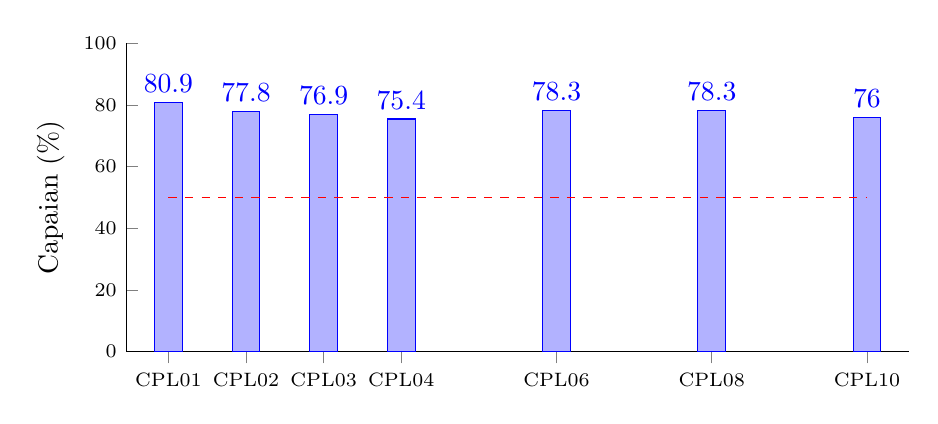
\begin{tikzpicture}
\begin{axis}[
  ybar, bar width=10pt, width=0.95\linewidth, height=5.5cm,
  ylabel={Capaian (\%)},
  symbolic x coords={CPL01,CPL02,CPL03,CPL04,CPL05,CPL06,CPL07,CPL08,CPL09,CPL10},
  xtick=data, nodes near coords, nodes near coords align={vertical},
  ymin=0, ymax=100, enlarge x limits=0.06,
  x tick label style={font=\scriptsize}, y tick label style={font=\scriptsize},
  axis lines*=left,
]
\addplot coordinates {(CPL01,80.9) (CPL02,77.8) (CPL03,76.9) (CPL04,75.4) (CPL06,78.3) (CPL08,78.3) (CPL10,76.0)};
\draw[dashed, red] (axis cs:CPL01,50.01) -- (axis cs:CPL10,50.01);
\end{axis}
\end{tikzpicture}
\hspace{0.5cm}
\begin{tikzpicture}
\begin{polaraxis}[
  width=6cm, height=6cm,
  xtick={0,36,72,108,144,180,216,252,288,324},
  xticklabels={CPL01,CPL02,CPL03,CPL04,CPL05,CPL06,CPL07,CPL08,CPL09,CPL10},
  tick label style={font=\scriptsize},
  ymin=0, ymax=100, ytick={0,25,50,75,100},
]
\addplot+[mark=*, thick, mark size=1.5pt] coordinates {(0,80.9) (36,77.8) (72,76.9) (108,75.4) (180,78.3) (252,78.3) (324,76.0) (0,80.9)};
\addplot[dashed, red, no markers] coordinates {(0,50.01) (36,50.01) (72,50.01) (108,50.01) (144,50.01) (180,50.01) (216,50.01) (252,50.01) (288,50.01) (324,50.01) (0,50.01)};
\end{polaraxis}
\end{tikzpicture}
\end{center}

\textbf{Angkatan 2019} --- 3.342 nilai; rata-rata lintas-CPL 73,9\%. Seluruh 10 CPL terukur. Capaian tertinggi pada CPL04 (77,2\%) dan CPL03 (75,3\%); terendah CPL09 (70,8\%) dan CPL05 (71,3\%). Seluruh CPL berada di atas 70\%.

\begin{center}
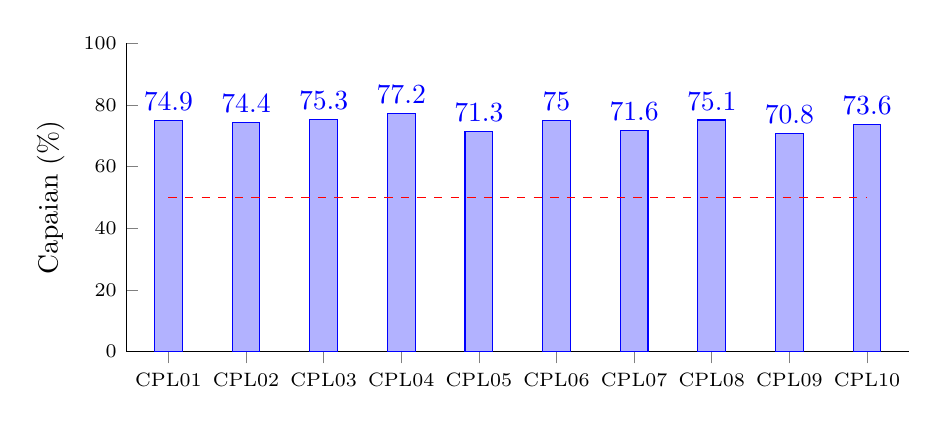
\begin{tikzpicture}
\begin{axis}[
  ybar, bar width=10pt, width=0.95\linewidth, height=5.5cm,
  ylabel={Capaian (\%)},
  symbolic x coords={CPL01,CPL02,CPL03,CPL04,CPL05,CPL06,CPL07,CPL08,CPL09,CPL10},
  xtick=data, nodes near coords, nodes near coords align={vertical},
  ymin=0, ymax=100, enlarge x limits=0.06,
  x tick label style={font=\scriptsize}, y tick label style={font=\scriptsize},
  axis lines*=left,
]
\addplot coordinates {(CPL01,74.9) (CPL02,74.4) (CPL03,75.3) (CPL04,77.2) (CPL05,71.3) (CPL06,75.0) (CPL07,71.6) (CPL08,75.1) (CPL09,70.8) (CPL10,73.6)};
\draw[dashed, red] (axis cs:CPL01,50.01) -- (axis cs:CPL10,50.01);
\end{axis}
\end{tikzpicture}
\hspace{0.5cm}
\begin{tikzpicture}
\begin{polaraxis}[
  width=6cm, height=6cm,
  xtick={0,36,72,108,144,180,216,252,288,324},
  xticklabels={CPL01,CPL02,CPL03,CPL04,CPL05,CPL06,CPL07,CPL08,CPL09,CPL10},
  tick label style={font=\scriptsize},
  ymin=0, ymax=100, ytick={0,25,50,75,100},
]
\addplot+[mark=*, thick, mark size=1.5pt] coordinates {(0,74.9) (36,74.4) (72,75.3) (108,77.2) (144,71.3) (180,75.0) (216,71.6) (252,75.1) (288,70.8) (324,73.6) (0,74.9)};
\addplot[dashed, red, no markers] coordinates {(0,50.01) (36,50.01) (72,50.01) (108,50.01) (144,50.01) (180,50.01) (216,50.01) (252,50.01) (288,50.01) (324,50.01) (0,50.01)};
\end{polaraxis}
\end{tikzpicture}
\end{center}

\textbf{Angkatan 2020} --- 5.492 nilai; rata-rata lintas-CPL 75,9\%. Seluruh 10 CPL terukur. Capaian tertinggi pada CPL08 (78,8\%) dan CPL03 (77,8\%); terendah CPL02 (73,1\%) dan CPL01 (74,0\%). Seluruh CPL berada di atas 70\%.

\begin{center}
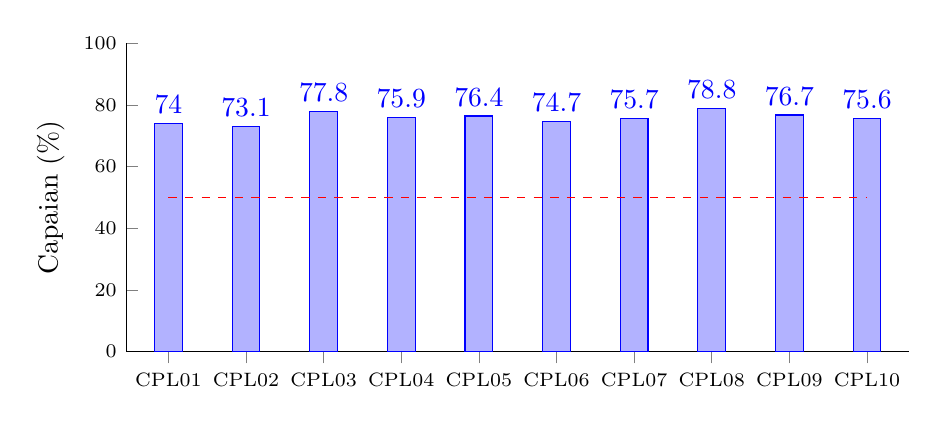
\begin{tikzpicture}
\begin{axis}[
  ybar, bar width=10pt, width=0.95\linewidth, height=5.5cm,
  ylabel={Capaian (\%)},
  symbolic x coords={CPL01,CPL02,CPL03,CPL04,CPL05,CPL06,CPL07,CPL08,CPL09,CPL10},
  xtick=data, nodes near coords, nodes near coords align={vertical},
  ymin=0, ymax=100, enlarge x limits=0.06,
  x tick label style={font=\scriptsize}, y tick label style={font=\scriptsize},
  axis lines*=left,
]
\addplot coordinates {(CPL01,74.0) (CPL02,73.1) (CPL03,77.8) (CPL04,75.9) (CPL05,76.4) (CPL06,74.7) (CPL07,75.7) (CPL08,78.8) (CPL09,76.7) (CPL10,75.6)};
\draw[dashed, red] (axis cs:CPL01,50.01) -- (axis cs:CPL10,50.01);
\end{axis}
\end{tikzpicture}
\hspace{0.5cm}
\begin{tikzpicture}
\begin{polaraxis}[
  width=6cm, height=6cm,
  xtick={0,36,72,108,144,180,216,252,288,324},
  xticklabels={CPL01,CPL02,CPL03,CPL04,CPL05,CPL06,CPL07,CPL08,CPL09,CPL10},
  tick label style={font=\scriptsize},
  ymin=0, ymax=100, ytick={0,25,50,75,100},
]
\addplot+[mark=*, thick, mark size=1.5pt] coordinates {(0,74.0) (36,73.1) (72,77.8) (108,75.9) (144,76.4) (180,74.7) (216,75.7) (252,78.8) (288,76.7) (324,75.6) (0,74.0)};
\addplot[dashed, red, no markers] coordinates {(0,50.01) (36,50.01) (72,50.01) (108,50.01) (144,50.01) (180,50.01) (216,50.01) (252,50.01) (288,50.01) (324,50.01) (0,50.01)};
\end{polaraxis}
\end{tikzpicture}
\end{center}

\textbf{Angkatan 2021} --- 6.904 nilai; rata-rata lintas-CPL 73,5\%. Seluruh 10 CPL terukur. Capaian tertinggi pada CPL05 (79,8\%) dan CPL01 (79,4\%); terendah CPL06 (66,6\%) dan CPL07 (68,4\%). Terdapat 5 CPL di bawah 70\% (CPL02, CPL06, CPL07, CPL08, CPL10) yang memerlukan perhatian.

\begin{center}
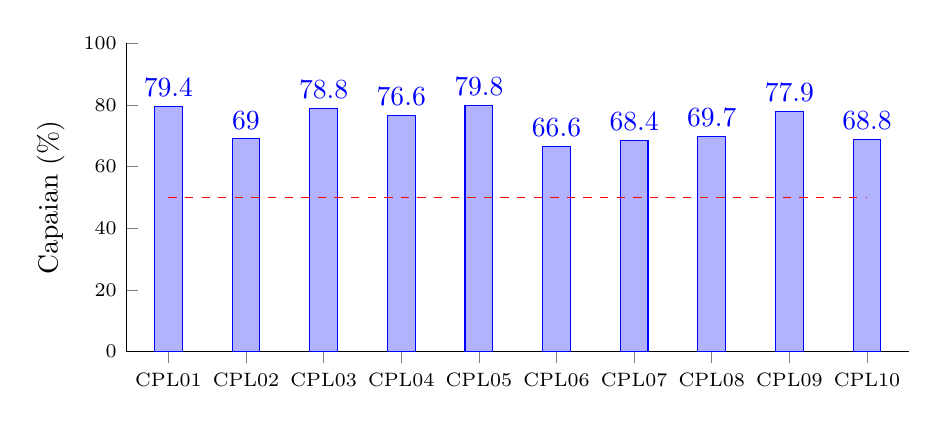
\begin{tikzpicture}
\begin{axis}[
  ybar, bar width=10pt, width=0.95\linewidth, height=5.5cm,
  ylabel={Capaian (\%)},
  symbolic x coords={CPL01,CPL02,CPL03,CPL04,CPL05,CPL06,CPL07,CPL08,CPL09,CPL10},
  xtick=data, nodes near coords, nodes near coords align={vertical},
  ymin=0, ymax=100, enlarge x limits=0.06,
  x tick label style={font=\scriptsize}, y tick label style={font=\scriptsize},
  axis lines*=left,
]
\addplot coordinates {(CPL01,79.4) (CPL02,69.0) (CPL03,78.8) (CPL04,76.6) (CPL05,79.8) (CPL06,66.6) (CPL07,68.4) (CPL08,69.7) (CPL09,77.9) (CPL10,68.8)};
\draw[dashed, red] (axis cs:CPL01,50.01) -- (axis cs:CPL10,50.01);
\end{axis}
\end{tikzpicture}
\hspace{0.5cm}
\begin{tikzpicture}
\begin{polaraxis}[
  width=6cm, height=6cm,
  xtick={0,36,72,108,144,180,216,252,288,324},
  xticklabels={CPL01,CPL02,CPL03,CPL04,CPL05,CPL06,CPL07,CPL08,CPL09,CPL10},
  tick label style={font=\scriptsize},
  ymin=0, ymax=100, ytick={0,25,50,75,100},
]
\addplot+[mark=*, thick, mark size=1.5pt] coordinates {(0,79.4) (36,69.0) (72,78.8) (108,76.6) (144,79.8) (180,66.6) (216,68.4) (252,69.7) (288,77.9) (324,68.8) (0,79.4)};
\addplot[dashed, red, no markers] coordinates {(0,50.01) (36,50.01) (72,50.01) (108,50.01) (144,50.01) (180,50.01) (216,50.01) (252,50.01) (288,50.01) (324,50.01) (0,50.01)};
\end{polaraxis}
\end{tikzpicture}
\end{center}

\textbf{Angkatan 2022} --- 2.032 nilai; rata-rata lintas-CPL 78,2\%. Baru 7/10 CPL terukur (CPL06, CPL08, CPL10 belum terukur). Capaian tertinggi pada CPL04 (81,9\%) dan CPL09 (79,6\%); terendah CPL07 (74,9\%) dan CPL01 (75,8\%). Seluruh CPL yang terukur berada di atas 70\%.

\begin{center}
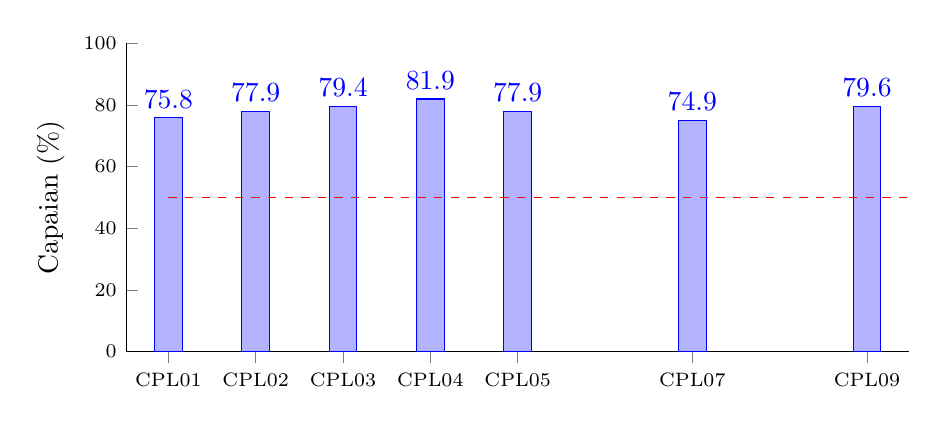
\begin{tikzpicture}
\begin{axis}[
  ybar, bar width=10pt, width=0.95\linewidth, height=5.5cm,
  ylabel={Capaian (\%)},
  symbolic x coords={CPL01,CPL02,CPL03,CPL04,CPL05,CPL06,CPL07,CPL08,CPL09,CPL10},
  xtick=data, nodes near coords, nodes near coords align={vertical},
  ymin=0, ymax=100, enlarge x limits=0.06,
  x tick label style={font=\scriptsize}, y tick label style={font=\scriptsize},
  axis lines*=left,
]
\addplot coordinates {(CPL01,75.8) (CPL02,77.9) (CPL03,79.4) (CPL04,81.9) (CPL05,77.9) (CPL07,74.9) (CPL09,79.6)};
\draw[dashed, red] (axis cs:CPL01,50.01) -- (axis cs:CPL10,50.01);
\end{axis}
\end{tikzpicture}
\hspace{0.5cm}
\begin{tikzpicture}
\begin{polaraxis}[
  width=6cm, height=6cm,
  xtick={0,36,72,108,144,180,216,252,288,324},
  xticklabels={CPL01,CPL02,CPL03,CPL04,CPL05,CPL06,CPL07,CPL08,CPL09,CPL10},
  tick label style={font=\scriptsize},
  ymin=0, ymax=100, ytick={0,25,50,75,100},
]
\addplot+[mark=*, thick, mark size=1.5pt] coordinates {(0,75.8) (36,77.9) (72,79.4) (108,81.9) (144,77.9) (216,74.9) (288,79.6) (0,75.8)};
\addplot[dashed, red, no markers] coordinates {(0,50.01) (36,50.01) (72,50.01) (108,50.01) (144,50.01) (180,50.01) (216,50.01) (252,50.01) (288,50.01) (324,50.01) (0,50.01)};
\end{polaraxis}
\end{tikzpicture}
\end{center}

\subsection{Agregat Semua Angkatan (Pooled)}

Agregat berikut bersifat \textit{pooled} atas seluruh 18.982 nilai lintas angkatan (lihat Metodologi); angkatan dengan observasi terbanyak (2021, 6.904 nilai) berpengaruh paling besar terhadap agregat ini.

\begin{center}
\begin{tabular}{L{2cm}C{2.6cm}C{2.6cm}C{2.4cm}}
\toprule
CPL & Rata-rata (\%) & \% $\geq$ 50,01 & $n$ observasi \\
\midrule
CPL01 & 77,8 & 99,9 & 2.848 \\
CPL02 & 71,7 & 92,6 & 9.706 \\
CPL03 & 77,3 & 99,8 & 11.886 \\
CPL04 & 77,8 & 98,5 & 1.359 \\
CPL05 & 75,4 & 98,7 & 6.133 \\
CPL06 & 72,4 & 92,8 & 11.274 \\
CPL07 & 71,8 & 94,0 & 6.346 \\
CPL08 & 76,4 & 97,7 & 6.520 \\
CPL09 & 77,8 & 99,3 & 5.414 \\
CPL10 & 73,1 & 94,3 & 5.813 \\
\bottomrule
\end{tabular}
\end{center}

\begin{center}
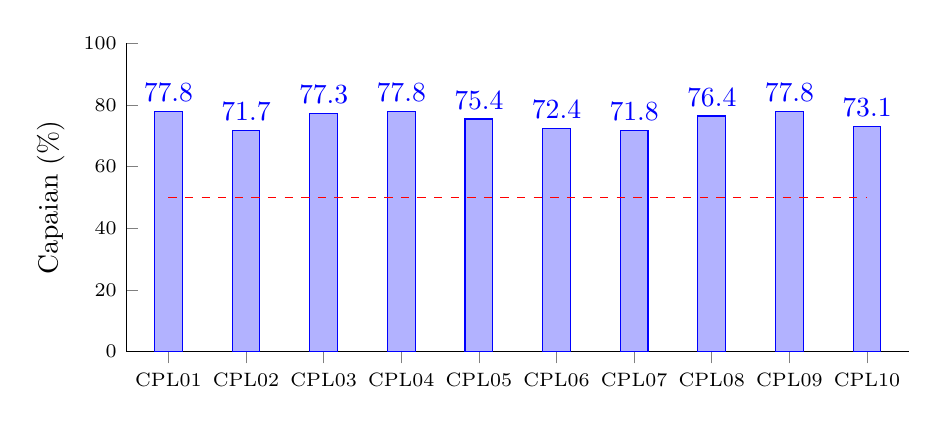
\begin{tikzpicture}
\begin{axis}[
  ybar, bar width=10pt, width=0.95\linewidth, height=5.5cm,
  ylabel={Capaian (\%)},
  symbolic x coords={CPL01,CPL02,CPL03,CPL04,CPL05,CPL06,CPL07,CPL08,CPL09,CPL10},
  xtick=data, nodes near coords, nodes near coords align={vertical},
  ymin=0, ymax=100, enlarge x limits=0.06,
  x tick label style={font=\scriptsize}, y tick label style={font=\scriptsize},
  axis lines*=left,
]
\addplot coordinates {(CPL01,77.8) (CPL02,71.7) (CPL03,77.3) (CPL04,77.8) (CPL05,75.4) (CPL06,72.4) (CPL07,71.8) (CPL08,76.4) (CPL09,77.8) (CPL10,73.1)};
\draw[dashed, red] (axis cs:CPL01,50.01) -- (axis cs:CPL10,50.01);
\end{axis}
\end{tikzpicture}
\hspace{0.5cm}
\begin{tikzpicture}
\begin{polaraxis}[
  width=6cm, height=6cm,
  xtick={0,36,72,108,144,180,216,252,288,324},
  xticklabels={CPL01,CPL02,CPL03,CPL04,CPL05,CPL06,CPL07,CPL08,CPL09,CPL10},
  tick label style={font=\scriptsize},
  ymin=0, ymax=100, ytick={0,25,50,75,100},
]
\addplot+[mark=*, thick, mark size=1.5pt] coordinates {(0,77.8) (36,71.7) (72,77.3) (108,77.8) (144,75.4) (180,72.4) (216,71.8) (252,76.4) (288,77.8) (324,73.1) (0,77.8)};
\addplot[dashed, red, no markers] coordinates {(0,50.01) (36,50.01) (72,50.01) (108,50.01) (144,50.01) (180,50.01) (216,50.01) (252,50.01) (288,50.01) (324,50.01) (0,50.01)};
\end{polaraxis}
\end{tikzpicture}
\end{center}

Rata-rata lintas-CPL pada agregat satu prodi adalah 75,1\%, dengan seluruh 10 CPL berada di atas 70\%. Capaian tertinggi pada CPL09 dan CPL04 (masing-masing 77,8\%); terendah pada CPL02 (71,7\%) dan CPL07 (71,8\%). CPL02, CPL06, CPL07, dan CPL10 konsisten berada pada capaian paling rendah di seluruh angkatan sehingga menjadi prioritas perbaikan berkelanjutan (\textit{Continuous Quality Improvement}, CQI) IABEE.

\subsection{Interpretasi dan Keterbatasan}
\label{subsec:cpl-keterbatasan}

Rata-rata capaian CPL berkisar antara 67\% dan 82\%; tingkat pencapaian ambang 50,01 sangat tinggi (92--99,9\%) karena ambang tersebut relatif rendah. CPL02, CPL06, CPL07, dan CPL10 relatif paling rendah secara konsisten dan menjadi kandidat utama fokus perbaikan berkelanjutan (CQI) IABEE.

Empat keterbatasan metodologis berikut wajib disertakan pada dokumen akreditasi:
\begin{enumerate}
\item Capaian bersifat agregat kohort anonim, bukan per-mahasiswa, sebagai akibat dari identitas data yang tercatat per-\textit{enrollment} (bukan per-NIM) pada basis data sumber.
\item Angkatan bersifat turunan (asumsi: digit awal kode kelas menunjukkan tingkat), dan belum divalidasi terhadap Nomor Induk Mahasiswa (NIM).
\item Pembobotan CPMK dilakukan dengan bagi rata, belum berbasis bobot RPS atau komponen asesmen yang sesungguhnya.
\item Nilai yang digunakan adalah satu skor akhir per mata kuliah (bukan per komponen penilaian); relasi mata kuliah dengan CPL mengikuti pemetaan Kurikulum 2025 pada \texttt{obe\_system}.
\end{enumerate}

Seluruh angka pada bagian ini bersifat \textit{read-only} dan belum diendapkan ke basis data produksi \texttt{obe\_system}. Analisis disusun dengan \textit{pipeline} \texttt{analyze\_cpp} (skrip introspeksi data, pemetaan mata kuliah, dan perhitungan capaian CPL), berbasis kerangka \textit{Outcome-Based Education} dan standar IABEE.
